\section{Parallel Logging}
Parallel logging uses multiple loggers and corresponding log files in order to improve the performance of the logging process. The concurrency control algorithm is used to ensure the serializability of the transactions that we have parsed into different threads. \par
A key insight of our parallel logging algorithm is how we handle the dependency between different transactions that operate on the same data tuples. There are four cases:
\begin{itemize}
\item Read-after-read dependency (RAR)
\item Read-after-write dependency (RAW)
\item Write-after-read dependency (WAR)
\item Write-after-write dependency (WAW)
\end{itemize}
RAR is equivalent to no dependency since no changes are made to the database. We discuss the rest of the cases using the following example, where cases of RAW, WAW and WAR are presented repectively in that order:
\begin{figure}[!h]
\caption{RAW, WAW and WAR dependencies}
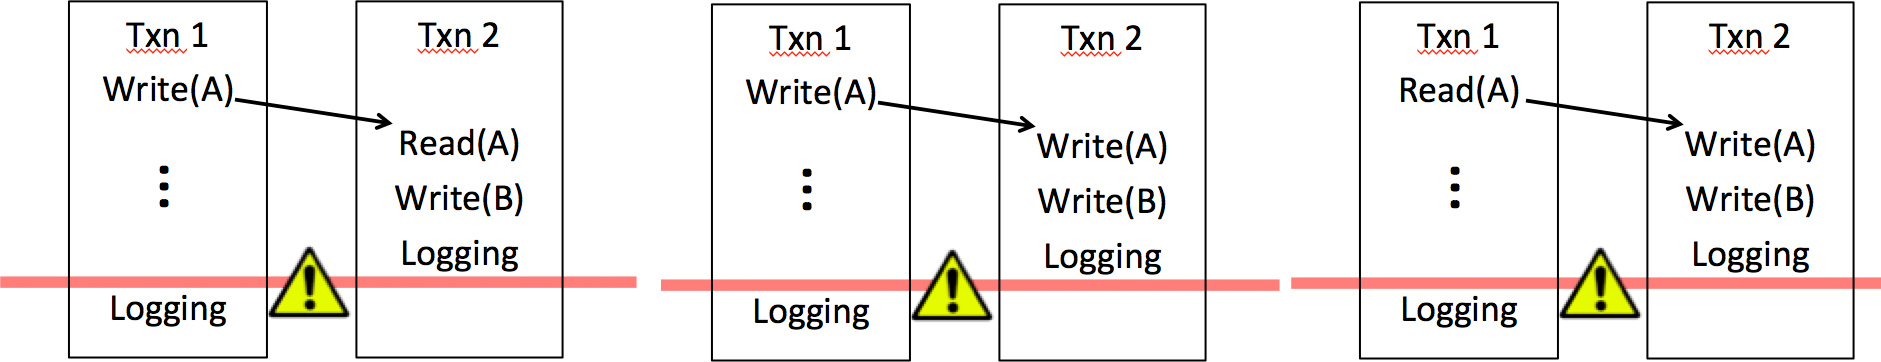
\includegraphics[width=\textwidth]{Dependencies.jpg}
\end{figure}\\
RAW dependency has to be maintained; if not, we may look at the first example. During recovery, the tuple A read by transaction 2 is not consistent with the value of A on the disk. 

Similarly, WAW has to be maintained; if not, we may look at the second example. During recovery, transaction 2 overwrites a phantom value of tuple A that cannot be tracked down in the system. 

We propose, however, that ignoring the WAR dependency, also known as  \textbf{anti-dependency}, will not affect the results of our task. This is demonstrated in the third example. In this case, there will be no conflicts in data consistency during recovery. Transaction 1 is simply lost, and all the values in the data tuples reflect the exact state of the system immediately before the crash. \par

Note that this will significantly decrease the time complexity of the logging algorithm because the number of writers to a data tuple is significantly smaller than the number of readers. In other words, transaction $A$ depends on the all the transactions before $A$ in the serializable order that write to $A$'s data tuples; therefore, $A$ can be logged once all the last writers to its data tuples have been logged. \par

To implement our algorithm, we specify the maximum log sequence number (LSN) in each log file that the transaction currently being logged depends on. When we attempt to log a transaction to the file, we compare the LSN that the transaction depends on ($A$) to the maximum LSN that has already been logged in each file ($B$). If $A\leq B$, the transaction is ready for logging; if $A>B$, we will push the transaction into a waiting queue after arbitrarily assigning it a LSN. The waiting queue will be checked periodically later on to see if any of its contents becomes ready for logging.\par

We use the following example to demonstrate the mechanism of our parallel logging algorithm: 
\begin{figure}[!h]
\caption{Example for Parallel Logging Algorithm}
\centering
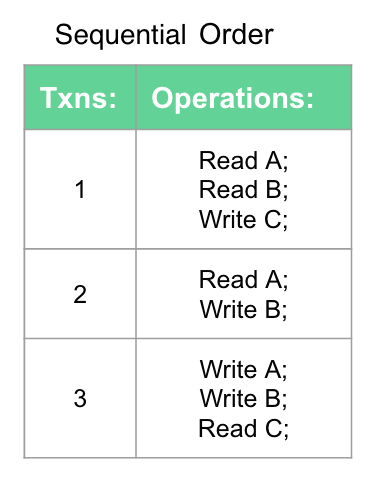
\includegraphics[width=100pt]{Parallel.png}
\end{figure}\par
If we use the serial logging algorithm, we are forced to log the three transactions one by one; when handling big data systems, this can be a serious bottleneck. Meanwhile, the parallel logging algorithm allows us to log multiple transactions. In this case, note that transactions 1 and 2 can be logged independently since tuple $A$ has no dependency and tuple $B$ is WAR, which, per our discussion above, allows for independent logging. Therefore, if transactions 1 and 2 are parsed into two different threads, they can both be logged without waiting. Transaction 3 depends on transaction 1 due to tuple $C$ (RAW) and on transaction 2 due to tuple $B$ (WAW), so it will be put into the waiting queue until both transaction 1 and 2 have already been logged. 
\begin{figure}[!h]
\caption{Example for Parallel Recovery}
\centering
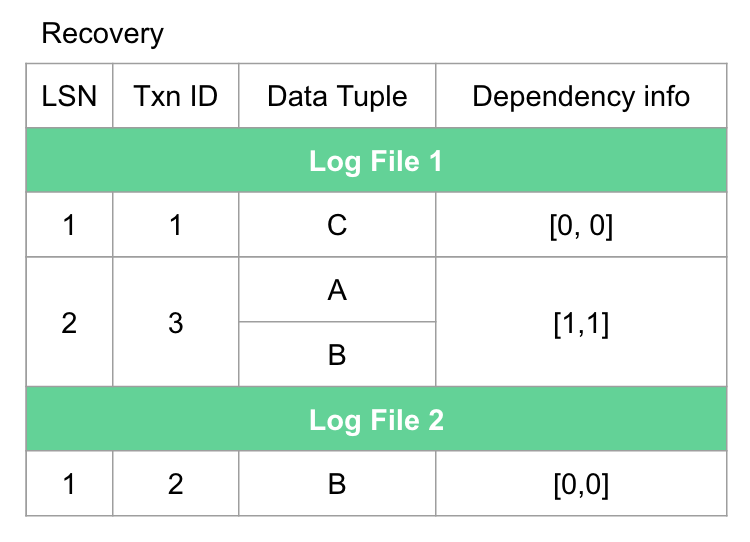
\includegraphics[width=150pt]{Parallel_re.png}
\end{figure}\par
We follow a similar process during recovery: we read the maximum LSN in each file that the current transaction depends on, and we compare it with the maximum LSN that has been recovered from that file. This ensures the serializability of the log records while improving the efficiency of the recovery process. In this particular example, two different threads take care of the two log files. While transactions 1 and 2 can be recovered immediately, transaction 3 is pushed into the waiting queue until both 1 and 2 have already been recovered.\par